% Vamos definir alguns comandos auxiliares para facilitar.

% "textbackslash" é muito comprido.
\newcommand{\sla}{\textbackslash}

% Vamos escrever comandos (como "make" ou "itemize") com formatação especial.
\newcommand{\cmd}[1]{\textsf{#1}}

% Idem para packages; aqui estamos usando a mesma formatação de \cmd,
% mas poderíamos escolher outra.
\newcommand{\pkg}[1]{\textsf{#1}}

% A maioria dos comandos LaTeX começa com "\"; vamos criar um
% comando que já coloca essa barra e formata com "\cmd".
\newcommand{\ltxcmd}[1]{\cmd{\sla{}#1}}

\chapter{Trabalhos Relacionados}
\label{chap:related_works}

Boa parte das pesquisas dedicada ao paralelismo
em compiladores é destinada ao desenvolvimento de compiladores que
paralelizam o código fonte fornecido automaticamente.
Há basicamente
duas áreas de estudo relacionadas a paralelização de compiladores, são
elas: análise de texto em paralelo e análise de fluxo de dados em paralelo.
Trabalhos dessas áreas também são apresentados em ordem cronológica nessa seção.

Dos algoritmos apresentados na Seção \ref{chap:fundamentacao}, o algoritmo
Recursivo Descendente é o mais simples deles. \cite{Lincoln:1970:PPT:987475.987478}
propôs a paralelização da análise léxica de um compilador
Fortran por meio da quebra do código fonte em partes menores. Para isso, o algoritmo proposto mapeia
informações de final de
linha e de posicionamento de cada caractere e realiza um processamento através de operações em APL.
Posteriormente, \cite{Krohn:1975:PAC:390015.808414} estendeu o trabalho
anterior, propondo uma maneira de realizar a análise sintática, a
tradução para a AST, e a geração
de código utilizando os registradores vetoriais do supercomputador
STAR-100. Ambos os artigos não apresentam nenhuma
análise assintótica para os algoritmos propostos, e tampouco apresentam
experimentos.

Posteriormente, \cite{Mickunas:1978:PCM:800127.804105} propôs uma
paralelização do algoritmo LR($0$). Sua ideia consiste em quebrar
arbitrariamente a entrada em vários segmentos e executar um analisador em paralelo
em cada um destes segmentos. Estes analisadores (exceto o primeiro,
que executa no início da entrada) são modificados na tentativa de
evitar conflitos, uma vez que modificar a ordem de início da análise
pode impossibilitar a distinção entre o prefixo e o sufixo de uma fase.
Quando um conflito é detectado, o analisador envia a sequência de
\textit{tokens} lida até então ao analisador à sua esquerda,
retorna ao estado inicial, e reinicia a sua análise.
No termino da análise, cada analisador envia o resultado para o analisador
a sua esquerda, acumulando o resultando no primeiro.
Os autores não mostraram experimentos ou
análise assintótica do algoritmo proposto. \cite{Pennello:1978:FMA:512760.512786}
implementou essa estratégia em um compilador Pascal, mas seus experimentos foram
realizados em um computador paralelo simulado.

\cite{vandevoorde1988parallel} paralelizou o \textit{Titan C compiler}, um compilador
C escrito em Modula-2. Sua implementação consiste na execução de um analisador léxico
em paralelo a um analisador sintático, sendo os \textit{tokens} alimentados
através de um \textit{pipeline}. O autor também propôs a paralelização de um
analisador sintático recursivo descendente que, após a sequência de declarações do programa, executa novas \textit{threads}
para cada expressão da gramática e tem
como premissa que qualquer declaração de funções do programa está no
cabeçalho do
arquivo. Essa estratégia de granularidade fina necessitou a implementação de
uma maneira de controlar o paralelismo, onde foi utilizado o conceito de
WorkCrews \citep{vandevoorde1988workcrews} que limita o número máximo de
\textit{threads} em execução simultânea. O autor relata um ganho de 10\% no
uso do \textit{pipeline} entre o analisador léxico e sintático, e um
\textit{speedup} de até $3.1\times$ utilizando 5 processadores MicroVAX II em
memória compartilhada. Entretanto, tal compilador não possui estágios de
otimização, e assim, métodos de paralelização de um otimizador não foram discutidos neste trabalho.

De maneira similar, \cite{wortman1992} implementou um compilador de Modula-2+
paralelo. A estratégia consiste em utilizar um analisador léxico capaz de
encontrar funções no código fonte e prosseguir com a compilação em paralelo
nesse nível, gerando uma tarefa para cada função. Para solucionar problemas
relacionados à chamada de funções e
acesso a símbolos ainda não definidos, o autor propõe o uso de
uma lógica ternária na tabela de símbolos, especificando um estado
``\textit{Doesn't know yet}'' (Ainda não visto), e propõe três estratégias para
implementar essa funcionalidade. Em seguida, o autor propõe o uso de
um número fixo de \textit{threads} trabalhadoras, e também o uso de uma fila de
prioridade produtor consumidor, onde as \textit{threads} deverão retirar o trabalho.
O uso de uma fila de prioridade permite que as funções mais longas sejam
processadas primeiro. Os experimentos conduzidos pelo autor mostraram
\textit{speedups} variando de $1.5\times$ até $6\times$ utilizando 8
processadores MicroVAX II em memória compartilhada.

Os artigos apresentados até então não abordam questões relacionadas
a otimização de código. Isso porque os compiladores naquela época possuíam poucos
passos de otimização, o que implicava em pouco tempo necessário para fazê-la.
Mesmo assim, alguns pesquisadores dedicaram-se a estudar esses passos.
\cite{Lee1994} explorou paralelismo na análise de controle
de fluxo. Como justificativa para esse estudo, os autores afirmam que a maior parte
do tempo gasto por compiladores otimizadores é com este tipo de análise,
principalmente nas otimizações Inter Procedurais. 
A investigação se concentrou em algoritmos que usam o grafo de controle
de fluxo como entrada. Os autores propõem uma heurística de aglutinação
para particionar tal grafo em regiões conexas e adjacentes de tamanho não maior
que um certo inteiro $s$. O uso da heurística é por razão do problema de
de particionamento ser NP-difícil.
Os experimentos da implementação utilizaram
8 processadores do computador iPSC/2 em memória distribuída, e 
obtiveram \textit{speedups} variando de
$2.8 \times$ até $6.5\times$. Os autores argumentaram que o \textit{speedup} foi
limitado devido às características dos programas no teste: os arquivos consistiam
de várias funções pequenas, o que normalmente é considerado uma boa prática de
programação.

Uma outra forma de explorar o paralelismo utilizando um Grafo Dirigido Acíclico
foi proposta por \cite{kramer1994combining}. Os autores mostram formas de propagar
em paralelo as informações nesse grafo explorando seus caminhos independentes,
e mostra uma maneira de transformar um Grafo de Controle de Fluxo com laços em
um Grafo de Controle de Fluxos acíclico equivalente. Os experimentos realizados
pelos autores apenas mostram oportunidades de paralelismo encontrada pelo
algoritmo.

Após estes resultados, houve um aparente hiato nas pesquisas relacionadas a
compilação em paralelo. As possíveis razões são a complexidade de um compilador
como programa, e o modelo dos processadores daquela época, que ainda eram
majoritariamente sequenciais. Uma década depois, houve uma explosão de processadores
paralelos e do poder computacional como um todo, como apresentado na Seção
\ref{sec:parallel_comp}. Este ganho computacional levou às empresas a propor soluções
ainda mais complexas para
gerar código mais eficiente. Embora apresentadas como maneiras de otimizar o código
dado como entrada, há relação nessas soluções com paralelismo em compiladores.

\cite{whoprgoogle} propuseram uma alteração no
compilador GCC com a finalidade
de possibilitar otimizações no programa como um todo. A alteração consiste
em construir um grafo de chamadas de função em relação a todo o programa,
ao contrário do modelo clássico, em que cada módulo é compilado independentemente.
Esse processo é composto por três etapas:
\begin{enumerate}
    \item \textit{Local Generation } (LGEN). Cada função do programa é compilada
        na Linguagem Intermediária, em conjunto com o grafo de chamadas de função.
        Esse estágio pode ser executado em paralelo.

    \item \textit{Whole Program Analysis} (WPA). O grafo de chamadas de função global
        é construído e as otimizações a serem efetuadas são selecionadas. Esse estágio
        deve ser executado sequencialmente.

    \item \textit{Local Transformations} (LTRANS). Todas as decisões aplicadas na
        etapa 2 são implementadas localmente e o código objeto final é gerado.
        Esse estágio pode executar em paralelo.
\end{enumerate}

A Figura \ref{fig:whopr_build} retrata este processo. Primeiro, cada arquivo é
compilado para a Linguagem Intermediária do Compilador (no GCC, a GIMPLE), em
conjunto com o seu Grafo de Chamadas de Função, gerando arquivos objeto
\texttt{lto\_obj*.o}. Esse passo ocorre em paralelo para cada arquivo. 
Em sequência, o gcc\_wpa é chamado, unindo todos os grafos
de chamada de função e decidindo como aplicar cada otimização Inter Procedural para
cada função do programa. Em seguida, o gcc\_ltrans é chamado para cada partição do
Grafo de Chamadas de Função, gerando os arquivos objetos para que o LD por
fim gere o binário final.

Essa proposta foi implementada
no GCC \citep{glek2010optimizing} com o nome de
\textit{Link Time Optimization} (LTO). A granularidade
escolhida na etapa LGEN foi paralelismo por arquivo. Já na LTRANS a granularidade
escolhida foram partições do arquivo objeto, o que possibilitou, como
consequência, a otimização de funções de um arquivo em paralelo. Os autores
testaram essa implementação com o
código fonte do Mozilla Firefox e do GCC, e relataram que o GCC construiu
binários menores e mais rápidos. Os autores relataram que essa implementação tornou
o processo de autocompilação do GCC duas vezes mais lenta,
mas que também houve um ganho de 20 minutos na compilação do Firefox. Em todos os
casos relatados, os passos de otimização Intra Procedural consumiu mais tempo.
\cite{livska2014optimizing} completa a análise dessa funcionalidade.
Um dos problemas encontrados foi o uso elevado de memória para carregar o grafo de
chamadas de função global necessário na fase WPA, que atingiu 12Gb na compilação do
Chromium e 15Gb na compilação do Kernel Linux. A maior crítica desse processo
foi o tempo necessário para recompilar todo o programa quando uma simples alteração
era efetuada em um único arquivo, o que inviabilizava um desenvolvimento incremental.

\begin{figure}
\tikzstyle{block} = [rectangle, draw, fill=white,
    text width=6em, text centered, rounded corners, node distance=3cm, auto, minimum height=2em]
\tikzstyle{line} = [draw, -latex]
\tikzstyle{cloud} = [draw, ellipse,fill=white, node distance=2cm,
    minimum height=2em]
\begin{center}
\scalebox{0.7}{
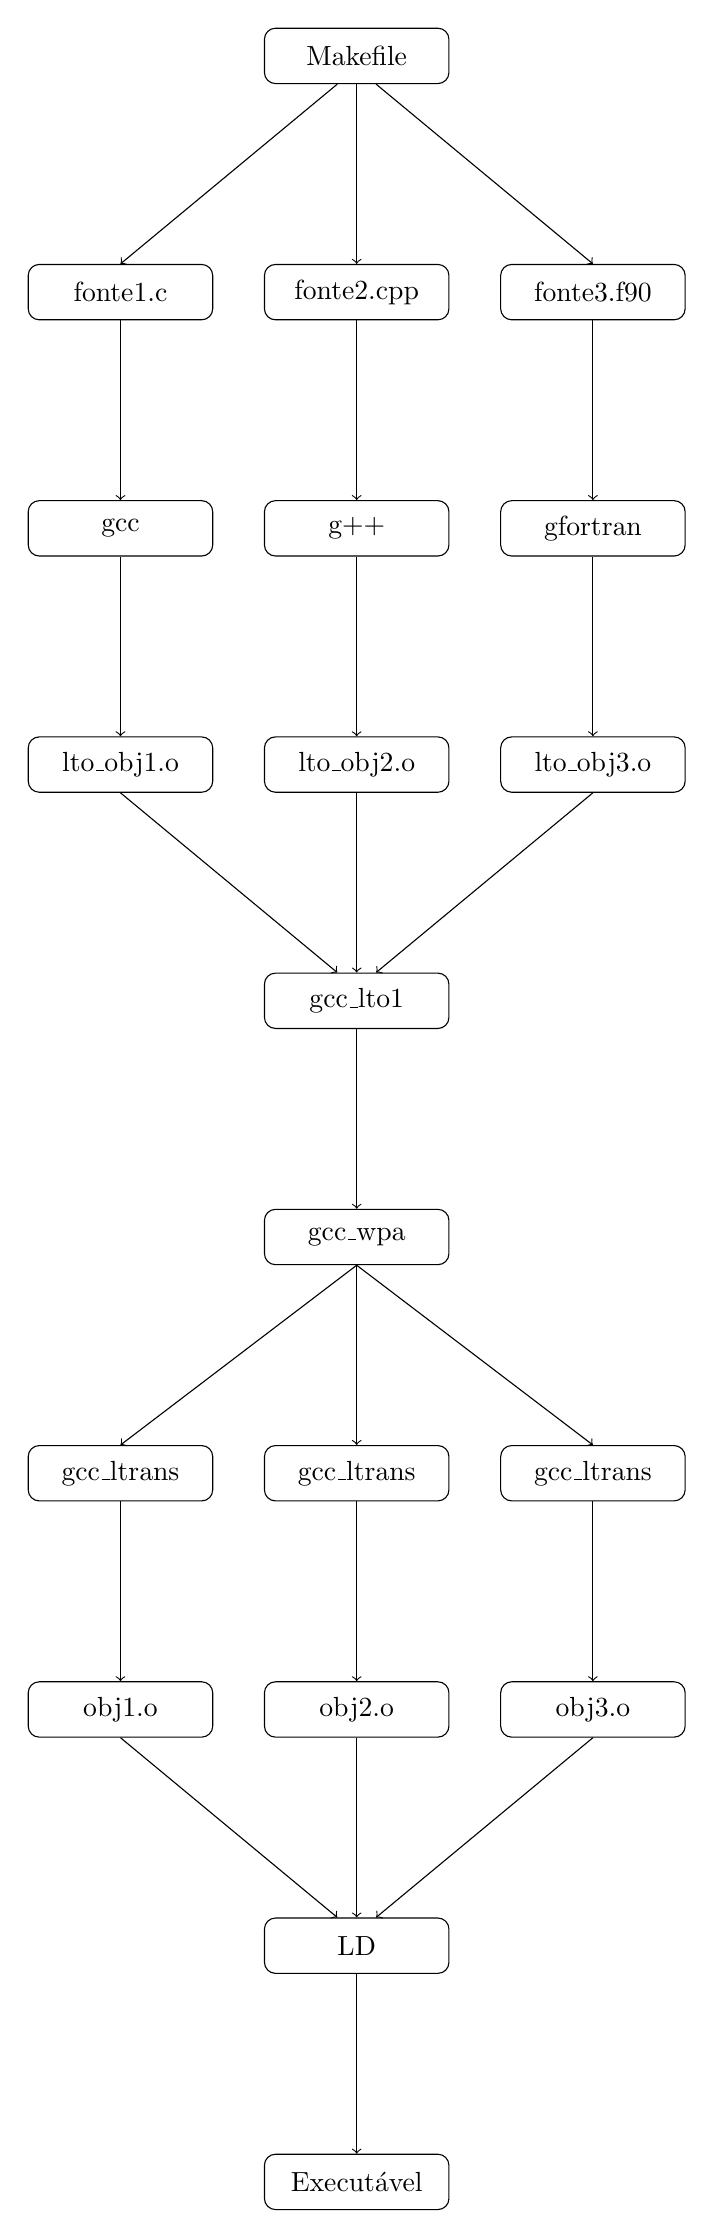
\begin{tikzpicture}[node distance = 3cm, auto]
    % Place nodes
    \node [block]                         (make)   {Makefile};
    \coordinate[below of=make]            (c);
    \node [block, left of=c]              (fonte1) {fonte1.c};
    \node [block, right of=fonte1]        (fonte2) {fonte2.cpp};
    \node [block, right of=fonte2]        (fonte3) {fonte3.f90};

    \node [block, below of=fonte1]        (gcc)      {gcc};
    \node [block, below of=fonte2]        (g++)      {g++};
    \node [block, below of=fonte3]        (gfortran) {gfortran};

    \node [block, below of=gcc]           (objeto1) {lto\_obj1.o};
    \node [block, below of=g++]           (objeto2) {lto\_obj2.o};
    \node [block, below of=gfortran]      (objeto3) {lto\_obj3.o};

    \node [block, below of=objeto2]       (gcc_lto) {gcc\_lto1};

    \node [block, below of=gcc_lto]       (gcc_wpa) {gcc\_wpa};
    \coordinate[below of=gcc_wpa]            (c2);

    \node [block, left of=c2]            (gcc_ltrans1) {gcc\_ltrans};
    \node [block, right of=gcc_ltrans1]   (gcc_ltrans2) {gcc\_ltrans};
    \node [block, right of=gcc_ltrans2]   (gcc_ltrans3) {gcc\_ltrans};

    \node [block, below of=gcc_ltrans1]   (obj1) {obj1.o};
    \node [block, below of=gcc_ltrans2]   (obj2) {obj2.o};
    \node [block, below of=gcc_ltrans3]   (obj3) {obj3.o};

    \node [block, below of=obj2]   (ld) {LD};

	\node [block, below of=ld]   (bin) {Executável};

    % Draw edges
    \draw[->]    ([xshift=-0.7em] make.south)   -- (fonte1.north);
    \draw[->]    (make.south)   -- (fonte2.north);
    \draw[->]    ([xshift=+0.7em] make.south)   -- (fonte3.north);

    \draw[->]    (fonte1.south)   -- (gcc.north);
    \draw[->]    (fonte2.south)   -- (g++.north);
    \draw[->]    (fonte3.south)   -- (gfortran.north);

    \draw[->]    (gcc.south)   -- (objeto1.north);
    \draw[->]    (g++.south)   -- (objeto2.north);
    \draw[->]    (gfortran.south)   -- (objeto3.north);

    \draw[->]    (objeto1.south)   -- ([xshift=-0.7em]gcc_lto.north);
    \draw[->]    (objeto2.south)   -- (gcc_lto.north);
    \draw[->]    (objeto3.south)   -- ([xshift=+0.7em]gcc_lto.north);

    \draw[->]    (gcc_lto.south)   -- (gcc_wpa.north);

    \draw[->]    (gcc_wpa.south)   -- (gcc_ltrans1.north);
    \draw[->]    (gcc_wpa.south)   -- (gcc_ltrans2.north);
    \draw[->]    (gcc_wpa.south)   -- (gcc_ltrans3.north);

    \draw[->]    (gcc_ltrans1.south)   -- (obj1.north);
    \draw[->]    (gcc_ltrans2.south)   -- (obj2.north);
    \draw[->]    (gcc_ltrans3.south)   -- (obj3.north);

    \draw[->]    (obj1.south)   -- ([xshift=-0.7em]ld.north);
    \draw[->]    (obj2.south)   -- (ld.north);
    \draw[->]    (obj3.south)   -- ([xshift=+0.7em]ld.north);

	\draw[->]    (ld.south)   -- (bin.north);


\end{tikzpicture}
}
\end{center}
\caption{Compilação de um programa utilizando WHOPR.}
\label{fig:whopr_build}
\end{figure}


Considerando o alto uso de memória e tempo de compilação nos casos relatados
acima, \cite{Johnson:2017:TSI:3049832.3049845} propôs o ThinLTO. A ideia é
considerar apenas parte do grafo global a cada vez, evitando carregá-lo
completamente na memória; e postergar ao máximo aplicar as otimizações possíveis,
realizando apenas análises de maneira sequencial e aplicando-as no 
\textit{backend} em paralelo.
Os autores relataram um \textit{speedup} de até $15\times$ quando comparado a
implementação do LTO original do Clang e até $4\times$ quando comparado a
implementação do LTO do GCC. Os autores também relataram uma diminuição considerável
no consumo de memória quando comparado ao LTO do GCC: Redução de 2.9Gb para 1Gb
na compilação do Clang, 10.8Gb para 1.0Gb no Chromium, e permitiu melhores otimizações no
\textit{Ad Delivery} da Google, enquanto a implementação do LTO no GCC
abortava a compilação após consumir mais de 25Gb de memória. O desempenho dos
binários gerados também foi similar, inclusive onde o LTO original gerava
binários mais lentos que o processo clássico de compilação. O tempo de compilação
também melhorou significativamente quando comparado ao LTO original,
mas permaneceu pior em todos os casos quando comparado ao processo clássico de
compilação.

Houve também nas pesquisas um renascimento de análise sintática em paralelo.
\cite{Barenghi:2015:PPM:2839536.2840146} encontrou uma maneira de explorar
a propriedade de Análise Local em Gramáticas com Precedência de Operadores.
Isso permitiu a construção de um gerador de analisadores sintáticos
PAPAGENO (\textit{Parallel Parser Generator}). Para isto, a gramática a
ser utilizada nesse analisador precisa ser convertida para uma Gramática
com Precedência de Operadores, conforme discutido e exemplificado pelos
autores. Testes empíricos foram efetuados implementando um analisador
JSON e outro analisador para a linguagem Lua. Em um Opteron 8378 (16 núcleos),
os autores atingiram um \textit{speedup} de até $5.3\times$ no análisador JSON
em arquivos grandes, e pouco mais de $4\times$ no analisador Lua. O algoritmo
paralelo foi comparado com os gerados pelo analisador sintático \textit{Bison},
que apenas gera código sequencial.


